\subsection{Non Programmable Privacy}

In addition to the Zcash team, other public blockchains that implement private transactions include Monero \cite{website:Monero}, Dash \cite{website:Dash}, Grin \cite{website:Grin}, and others. However, these public chains lack programmability and can only be used for simple private transfer of assets. Consequently, their ecosystem development lags far behind Ethereum, which has become the largest public chain in the ecosystem due to its programmability, but Ethereum lacks privacy features.

Therefore, some projects have begun to explore ways to introduce privacy to Ethereum, such as the ZK-ZKRollup application zk.money \cite{website:zk.money} developed by the Aztec \cite{website:Aztec} team. However, the current zk.money product has been discontinued, mainly because it's privacy features only apply to simple single transfer scenarios. Given the current explosion of Defi applications, asset transfer is only one of the simplest financial scenarios, and therefore the user base is limited, while the maintenance costs continue to accrue.
\begin{figure}[!ht]
    \centering
    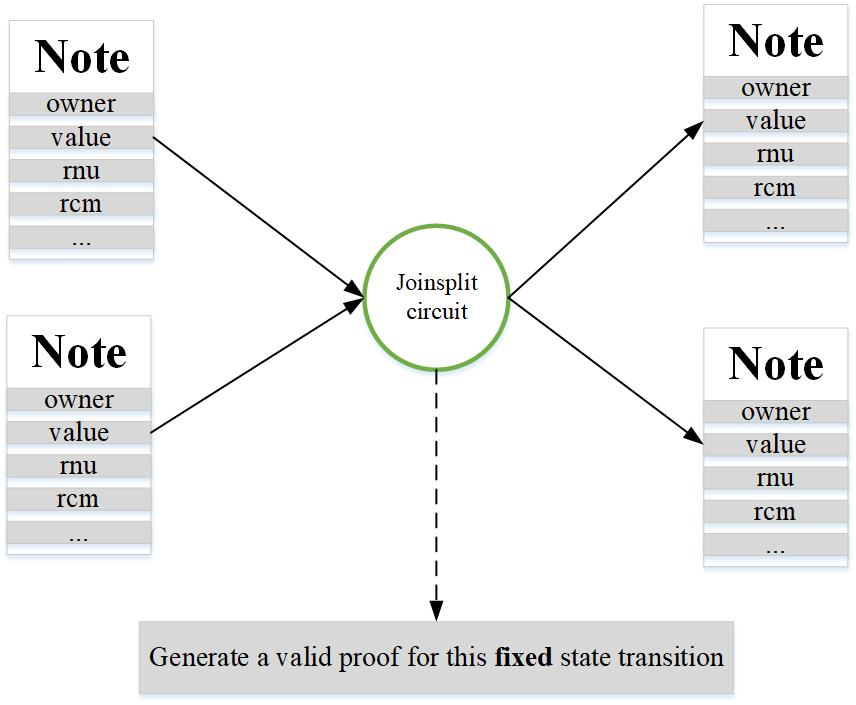
\includegraphics[width=0.4\textwidth]{Example of Non Programmable privacy.jpg}
    \caption{Example of Non Programmable Privacy}
    \label{fig:Example of Non Programmable Privacy}
\end{figure}

\figref{fig:Example of Non Programmable privacy} shows the simple logic of non programmable privacy. The value change logic corresponding to the input and output notes in Section \ref{section: sending-notes} are also fixed, generally in the form of ``A + B = C + D''. Manta Network \cite{website:Manta-network} is a public blockchain that supports user-defined token privacy transfers, and the privacy transaction 
constraint circuits of all fungible tokens can be used to reuse the above logic.

A ZK-ZKRollup application of a single scenario use case, is similar to a ZKRollup application of a single scenario use case. If you want to use the asset in other applications or for other use cases, you must cross the asset to another application through a bridge, which brings with it very poor user experience. Therefore, just as ZKRollups need to 
transition to ZK(E)VMs, ZK-ZKRollup also need to transition to ZK-ZKVMs (Appendix \ref{section: solidity-compatibility} explains how to get solidity compatibility).
